\section{Finite Element Analysis}

\indent

Finite element analysis was used to predict the load-bearing capacity and failure behavior of the sample bridge specimen under the compressive load. The \textit{ANSYS Composite PrepPost} (ACP) package of \textit{ANSYS} finite element software was utilized due to suggestion of Cooper Union faculty\footnote{Professor Scott Bondi suggested that this software be used since he is familiar with package and could provided guidance.} and ease of access with Cooper Union's existing \textit{ANSYS} license. The following subsections primarily focus on FEA results and conclusions that can be drawn from the numerical analysis. However, rigorous explainations of the finite element models and physics models utilized in this study are located in the Appendix.\\

\subsection{Finite Element Formulation}

\indent

ACP finite element modeling uses shell elements with orthotropic material properties to discretize geometry. The number of layers and thickness of each layer, which can be constant or variable, are assigned values. These parameters determine the overall thickness of each shell elemement, as well as the number of and spacing between integration points along the depth of each element. As such, the geometry input of ACP is a surface rather than a solid body. A reference direction is created within the model so that orthotropic element properties can be oriented accordingly with one direction representing the fiber, and other two being the matrix. In solving the model, Puck's failure criterion was used\footnote{The Tsai-Wu failure criterion was also considered due to its high frequency of appearance in research papers investigating carbon fiber 3D printing and curved layer 3D printing in general. However, Tsai-Wu failure was ultimately neglected since it required bi-axial stress data of the proposed filament, which could not easily be obtained.}. Puck failure is a phenomenological failure mode specifically suited for uni-direction (UD) CFRPs and glass fiber reinforced polymers (GFRPs) where inter-fiber failure\footnote{Failure of the matrix material, in shear, compression, or tension in a plane parallel to a plane contraining UD fibers.} (IFF) is most likely, which makes it the optimal failure mode for the FEA of the bridge specimen. Additionally, Puck Failure is intended for use with modeling IFF \large{\textbf{CITE}}. Table~\ref{fig:fea-bridge-speciment} shows the specific dimesions of the bridge geometry used in this analysis.\\

\begin{figure}[htp]
\centering
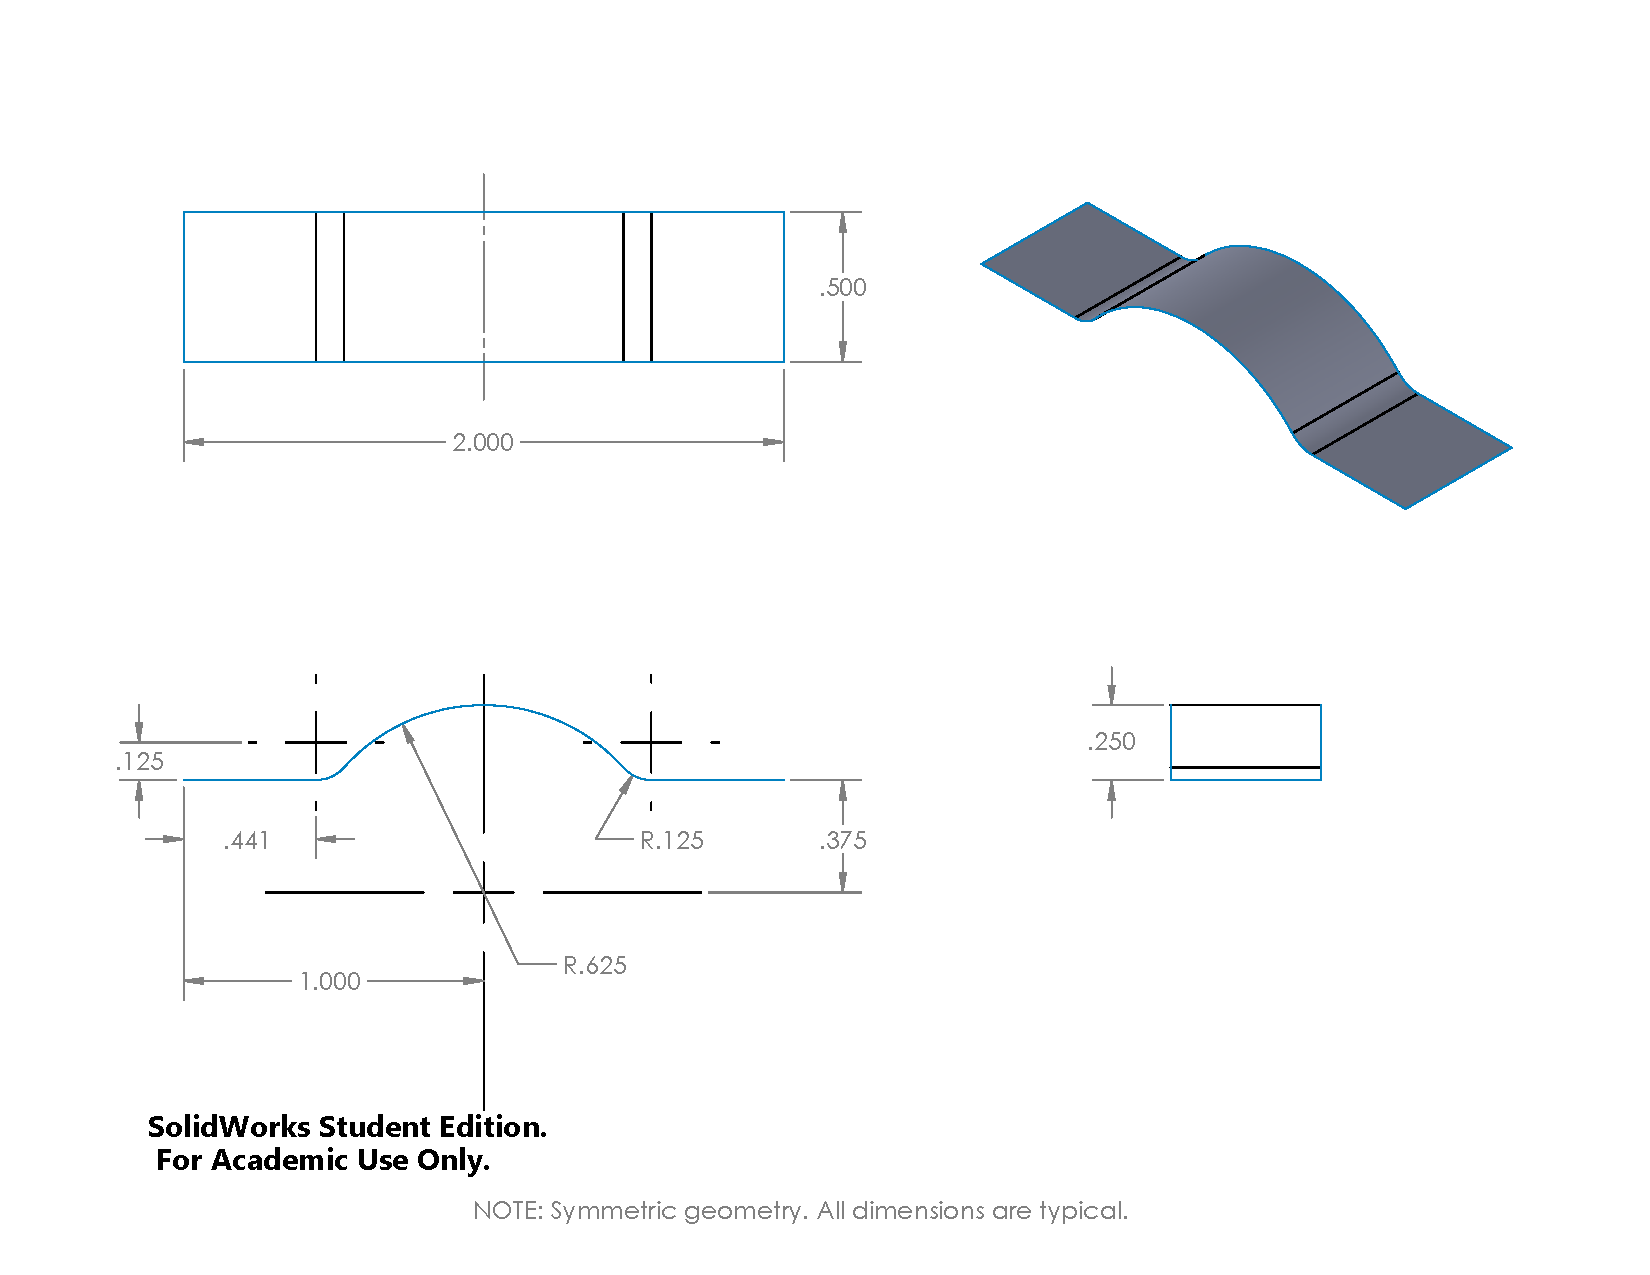
\includegraphics[width=1\textwidth]{./figures/fea/fea-surface-geometry}
\caption{The surface geometry used in ACP.}
\label{fig:fea-bridge-speciment}
\end{figure}

\clearpage

\subsection{ACP Results}

\indent

Figure~\ref{fig:fea-acp-tot-def} through Figure~\ref{fig:fea-acp-z-def} show the total and directional displacements of the loaded CFRP specimen loaded at 90 pounds-force, which puts the specimen just shy of failure. The units are in meters. Notable defection results are that the x-displacement of the loaded edge is on the same order of magnitude of the z-displacement of the central bend. Furthermore, the edges of the main bend warp slightly inward when the specimen is compressed (y-displacement).

%% Deformation

\begin{figure}[htp]
\centering
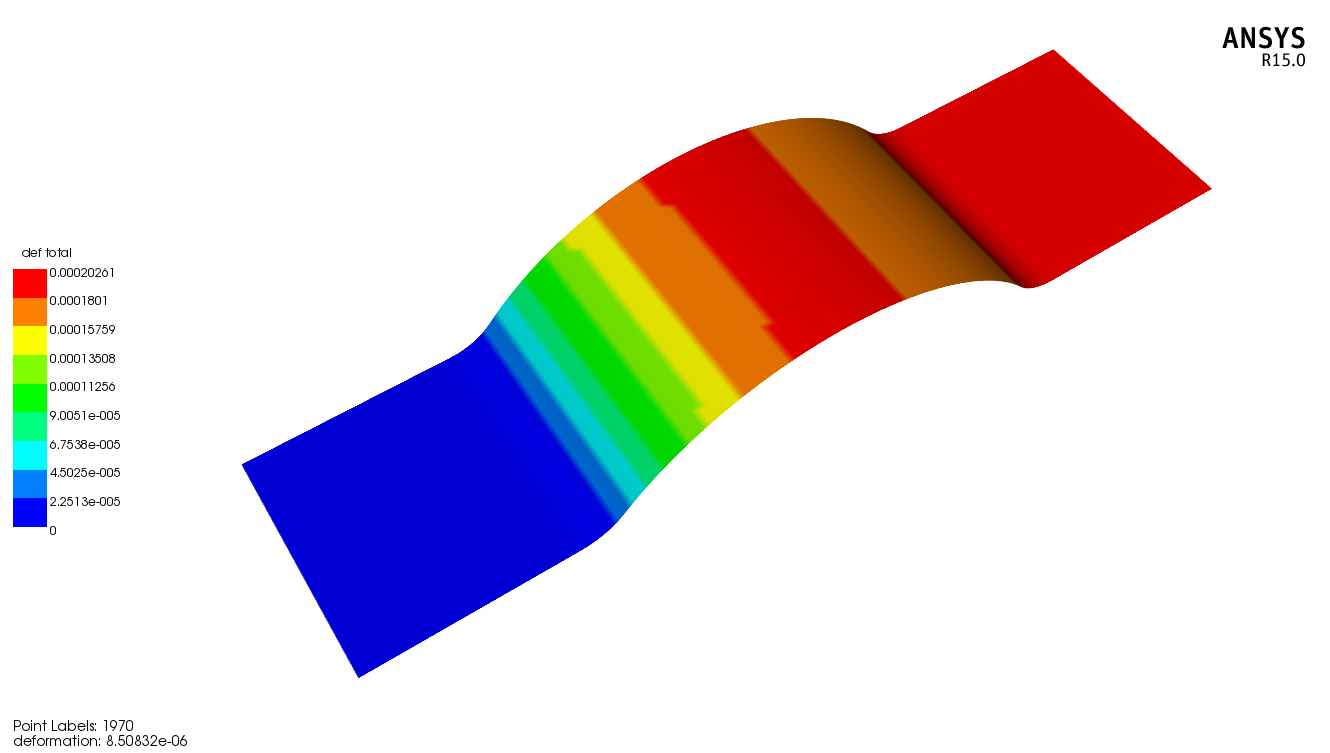
\includegraphics[width=1\textwidth]{./figures/fea/fea-acp-tot-def}
\caption{Total displacement FEA result.}
\label{fig:fea-acp-tot-def}
\end{figure}

\begin{figure}[htp]
\centering
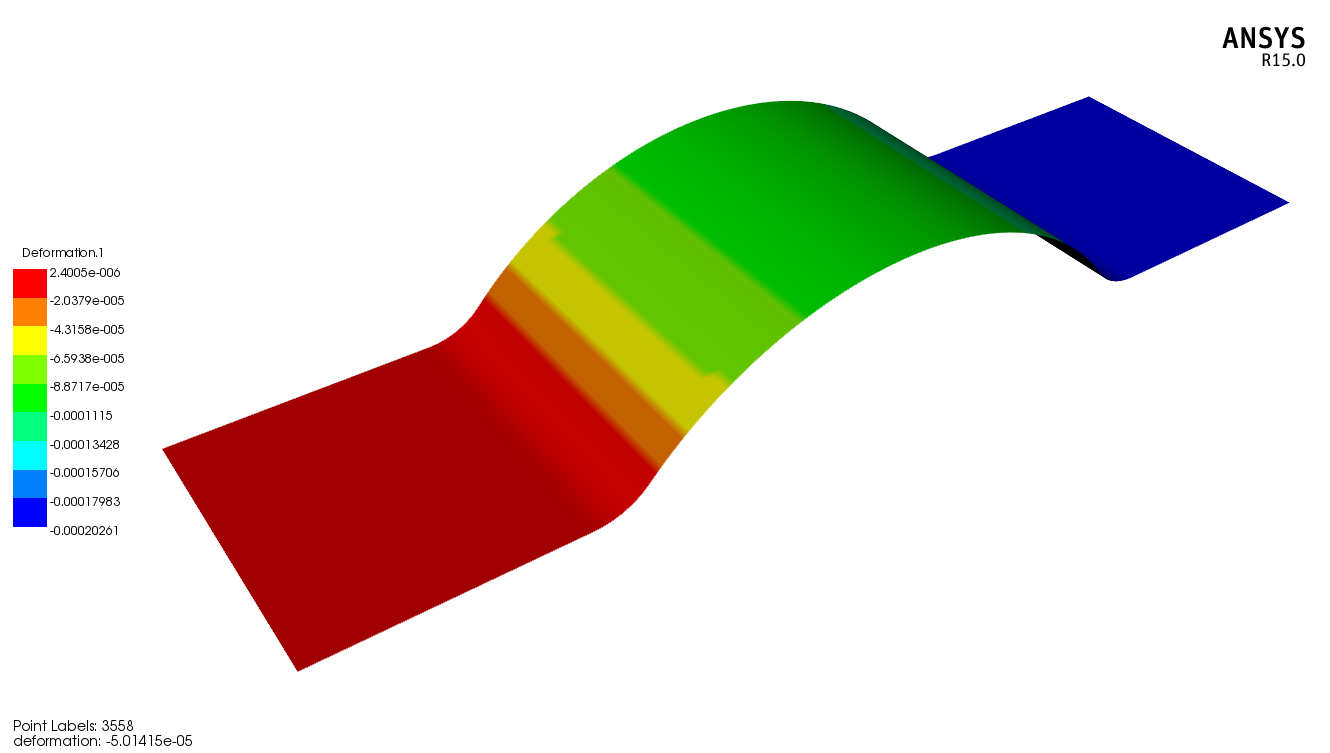
\includegraphics[width=1\textwidth]{./figures/fea/fea-acp-x-def}
\caption{X direction displacement FEA result.}
\label{fig:fea-acp-x-def}
\end{figure}

\begin{figure}[htp]
\centering
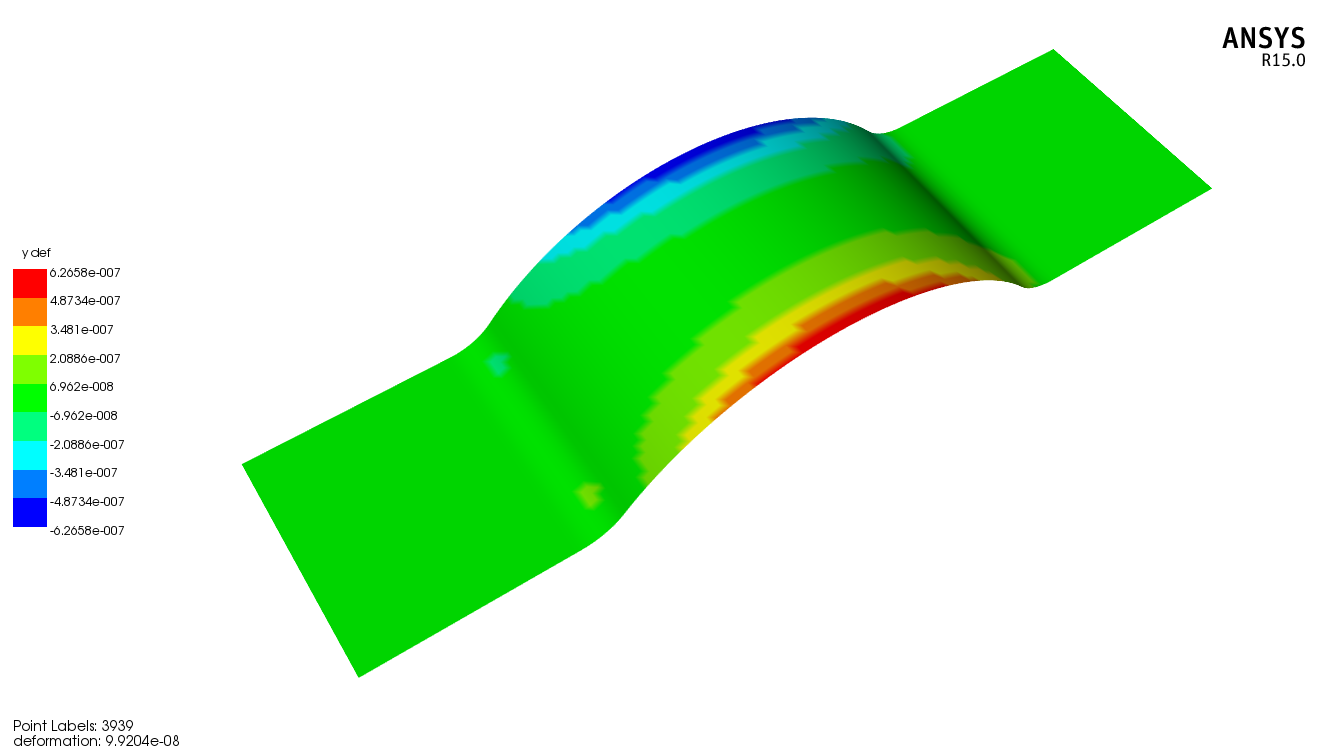
\includegraphics[width=1\textwidth]{./figures/fea/fea-acp-y-def}
\caption{Y direction displacement FEA result.}
\label{fig:fea-acp-y-def}
\end{figure}

\begin{figure}[htp]
\centering
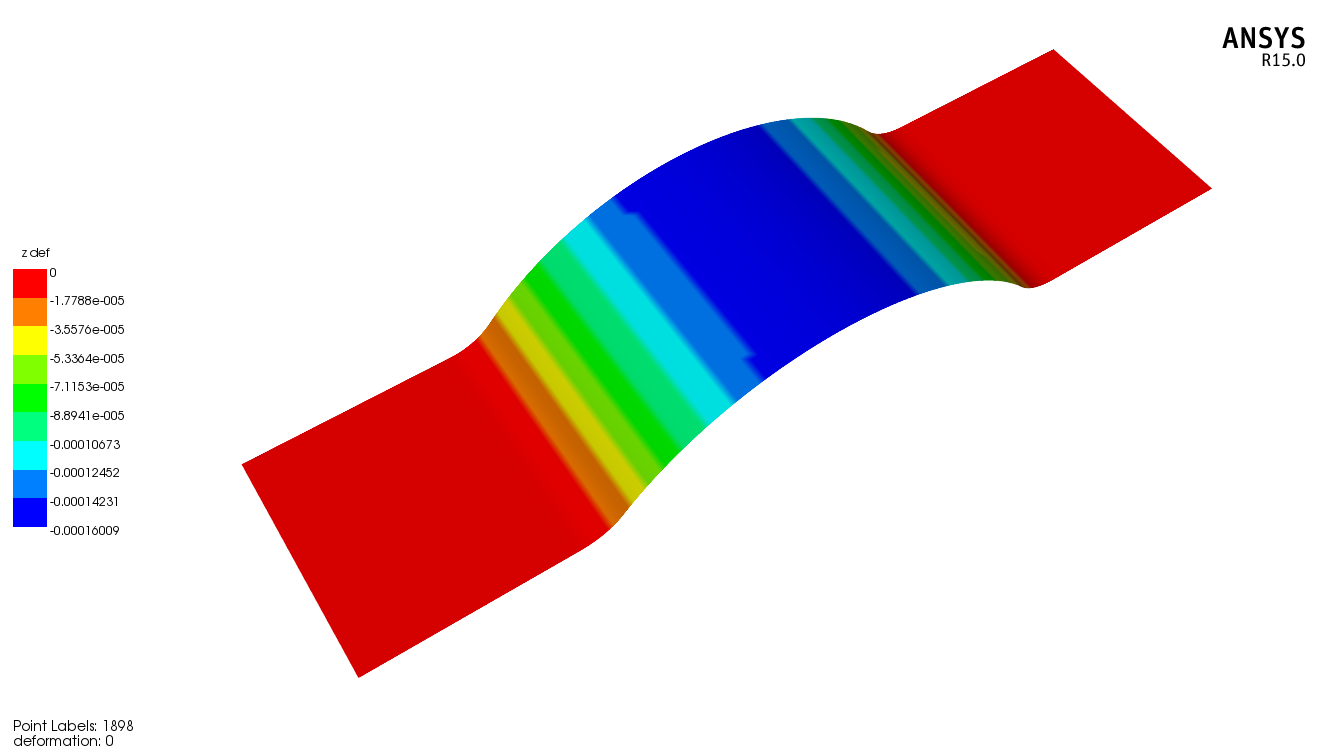
\includegraphics[width=1\textwidth]{./figures/fea/fea-acp-z-def}
\caption{Mesh overview of the composite model in \textit{ACP} with a solid-body display state applied.}
\label{fig:fea-acp-z-def}
\end{figure}

\clearpage

%%% Puck Failure Results

Figure~\ref{fig:fea-acp-pfailure-notext} shows the resulting Puck failure. A value of 1 or above (red) indicates failure. While the two small fillets in the geometry see localized small spikes in value compared to their neighbors, the area of main concern is the central bend. Similar to the trends of typical mechanics of materials concepts, this section of the geometry experiences the largest bending moment of the entire body and is therefore most susceptible to failure. Figure~\ref{fig:fea-acp-pfailure-layer-closeup} shows a close-up of the critical portion of the geometry with the critical layer displayed above each element. Note that the bottom layer (ply 1) of the flat geometry and fillet is the failing layer. Just after the fillet, transitioning into the main curve, the middle layer (ply 30) is of main concern. Finally, the center of the specimen fails at the top layer (ply 60). Using concepts from bending in mechanics of materials, it is apparent that layers in bending tension are critical. Figure~\ref{fig:fea-acp-pfailure-mode-closeup} shows the same close-up but with failure mode information displayed on each element (\emph{pmC} denotes matrix shear failure, and \emph{pd} signifies delamination). Therefore, the mode of failure for this bridge specimen is matrix shear, which is then followed by delamination and additional matrix shearing. Note that near the boundaries of the part (the fixed edge and loaded edge), the specimen does not experience failure, it is mainly localized to the central arch.

\begin{figure}[htp]
\centering
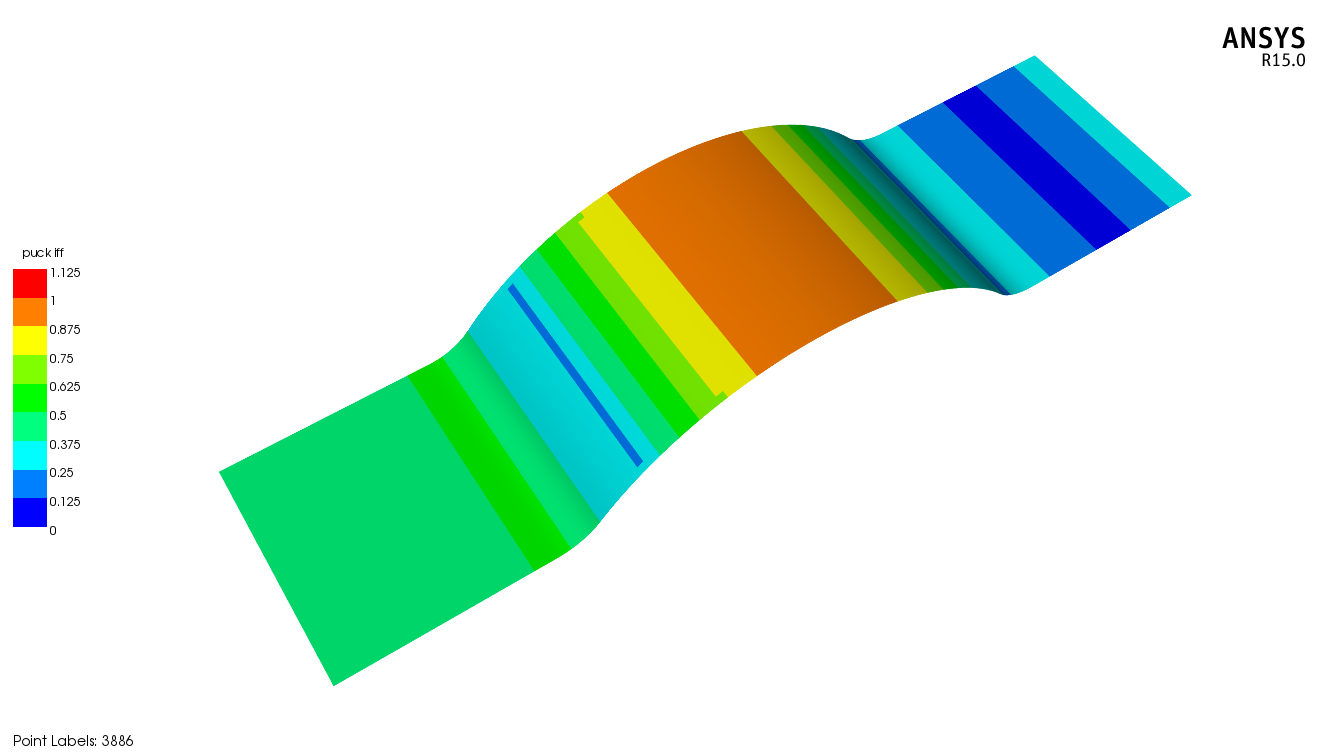
\includegraphics[width=1\textwidth]{./figures/fea/fea-acp-pfailure-notext}
\caption{Puck Failure contour plot.}
\label{fig:fea-acp-pfailure-notext}
\end{figure}

\begin{figure}[htp]
\centering
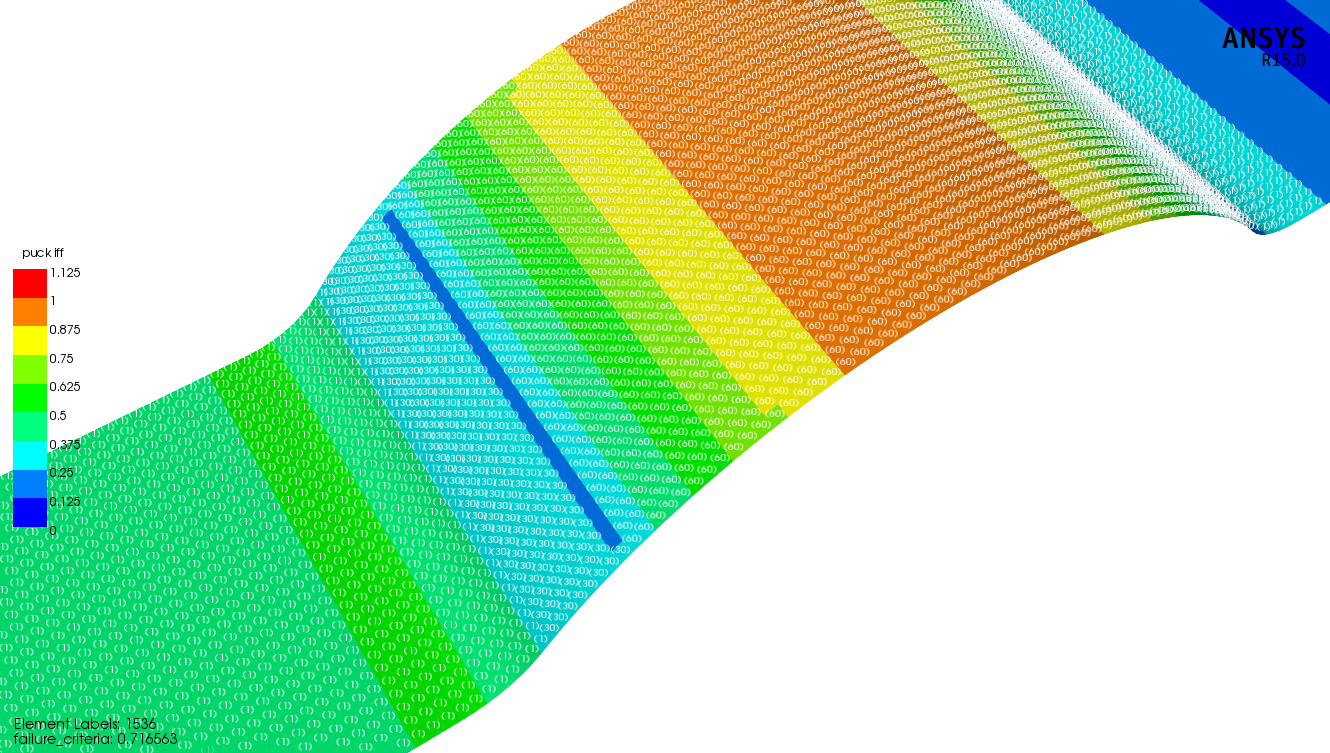
\includegraphics[width=1\textwidth]{./figures/fea/fea-acp-pfailure-layer-closeup}
\caption{Closeup of Puck Failure contour plot with tabulated failing layer.}
\label{fig:fea-acp-pfailure-layer-closeup}
\end{figure}

\begin{figure}[htp]
\centering
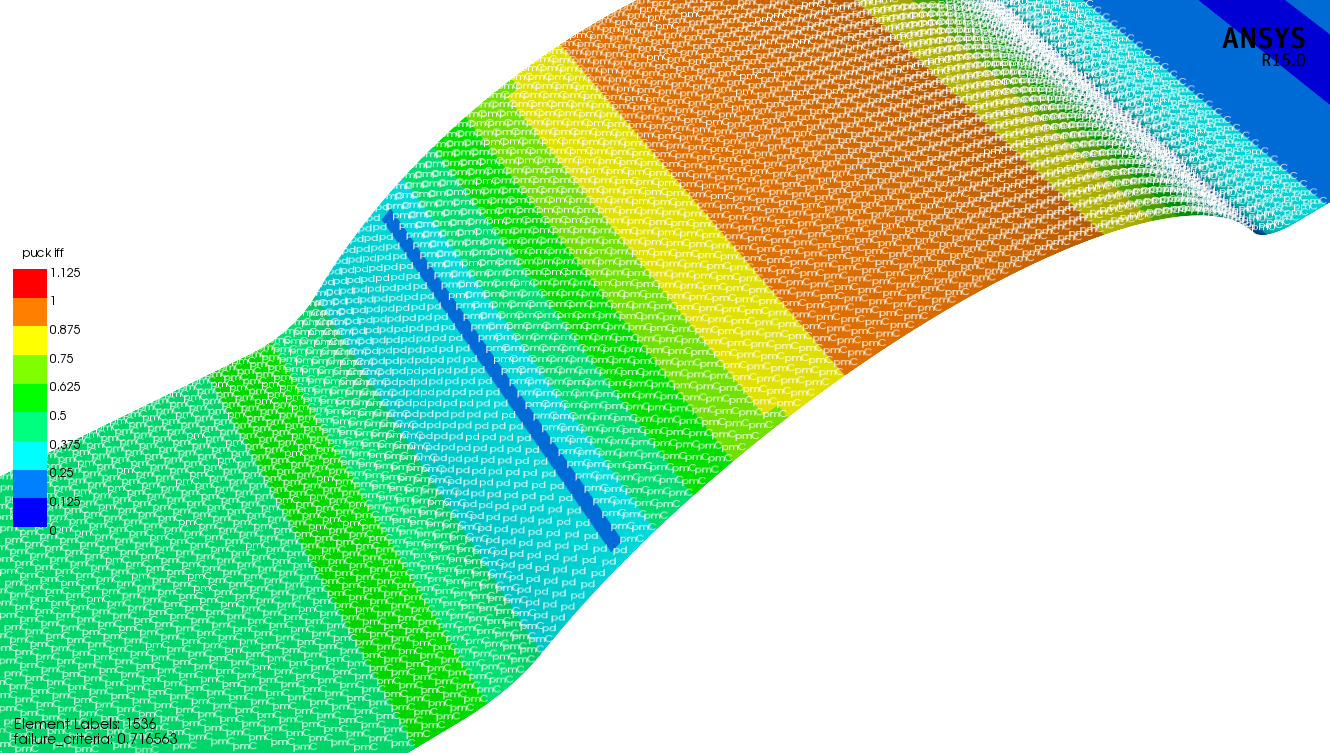
\includegraphics[width=1\textwidth]{./figures/fea/fea-acp-pfailure-mode-closeup}
\caption{Closeup of Puck Failure contour plot with tabulated failure modes.}
\label{fig:fea-acp-pfailure-mode-closeup}
\end{figure}

\clearpage

\subsection{Comparison to Puck Failure Criterion}

\indent

Methods of composite failure are very specific to fiber and matrix material properties, and to the micromechanics of the fiber-matrix structure. This makes a mathematical validation of FEA results nearly impossible with limited knowledge of the CFRP filament and 3D printed structure. However, qualitative trends from Puck's failure theory confirm the FEA findings.\\

Puck theorizes that $\theta_{fp} = 0^{\circ}$ transverse tension, $\theta_{fp} = 90^{\circ}$ through-thickness tension, $\theta_{fp} = 0^{\circ}$ positive inplane shear, $\theta_{fp} = 0^{\circ}$ negative inplane shear, $\theta_{fp} = 90^{\circ}$ positive transverse shear, $\theta_{fp} = 90^{\circ}$ negative transverse shear, $\theta_{fp} = +45^{\circ}$ positive through-thickness shear, and $\theta_{fp} = +45^{\circ}$ negative through-thickness shear are the fracture planes with the most significant impact on load bearing capacity of UD 3D geometry \large{\textbf{CITE}}. Logically then, the primary mode(s) of failure predicted for the bridge specimen should correlate to one or more of these IFF scenarios. Figure~\ref{fig:puck-failure-qualitative} shows the the loading of individual elements within the model that correlate to $\theta_{fp} = 90^{\circ}$ positive transverse shear (\emph{a}) and $\theta_{fp} = 90^{\circ}$ through-thickness tension (\emph{b}). Element \emph{a} shows a central bridge piece, which is in bending tension. The element adjacently left pulls mainly horizontally and slightly downward due to the curvature of the piece. Within the examined element, these forces are reacted to create a positive transverse shear load with a $90^{\circ}$ fracture plane (light grey) parallel to the fibers (dark grey). This failure mode is by the same reasoning evident in the portion of the fillet experiencing tension. Element \emph{b} depicts and element in the middle ply between the two curves. Since elements to its upper right, and bottom left are are in tension, the examined element is bi-axially loaded. The large horizonatl load is reacted by the strong fibers while the matrix then experiences vertical tensions and completely separates in delamination, which is characteristic of the $\theta_{fp} = 90^{\circ}$ through-thickness tension failure mode. Therefore, qualitative analysis of the specimen using Puck's failure theory agree with finite element results.\\

\begin{figure}[htp]
\centering
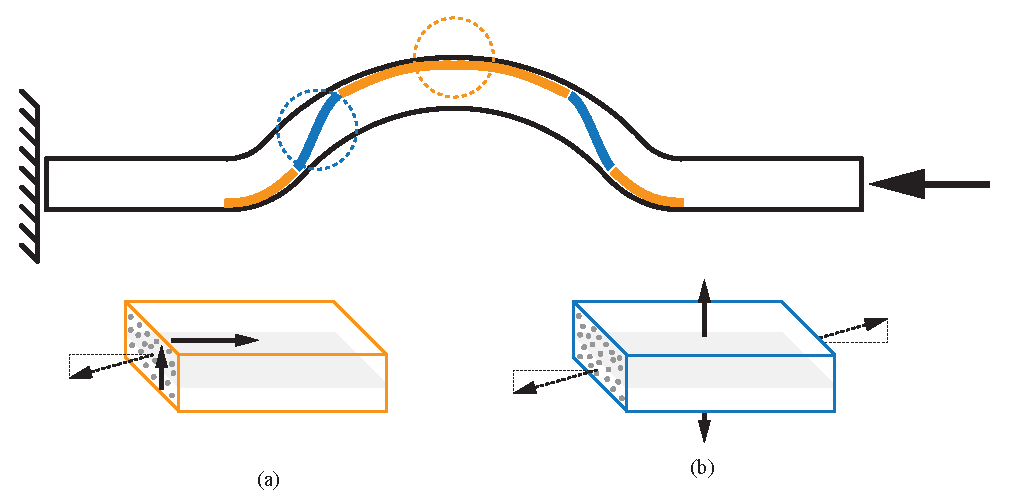
\includegraphics[width=1\textwidth]{./figures/fea/puck-failure-qualitative}
\caption{Diagrams of Puck IFF in the bridge specimen.}
\label{fig:puck-failure-qualitative}
\end{figure}

\clearpage

\subsection{Comparison to Aluminum and ABS}

\indent

For comparison, standard solid-body finite element analyses were also performed with the materials properties of ABS and aluminum under the same 90 pound-force compressive load from the CFRP study. The setup of these finite element models, as well as contour plots of the results are located in the Appendix. The factor of safety and the absolute values of directional deformations are located in Table~\ref{tab:fea-cfrp-al-abs}. The factor of safety assigned to the CFRP part is unity due to utilizing a load that puts the piece on the brink of failure. Following this convention, a positive factor of safety in another material denotes the margin that the load can be increased prior to reaching the ultimate tensile stress of the material. Similarly, a negative value indicates the margin by which the ultimate strength is surpassed by the applied load.

\begin{table}[htp]
    \centering
    \begin{tabular}{lcccc}
    
        Material & Factor of Safety & X Displacement, \emph{in} & Y Displacement, \emph{in} & Z Displacement, \emph{in} \\ \hline
        CFRP & 1 & 9.4E-05 & 2.5E-05 & 6.2E-03 \\
        Aluminum & 3.1 & 3.5E-05 & 5.9E-05 & 1.3E-05 \\
        ABS & 0.6 & N/A & N/A & N/A \\
                
    \end{tabular}
    \caption{Summary of CFRP, ABS, and aluminum FEA results.}
    \label{tab:fea-cfrp-al-abs}
\end{table}

The results show that a solid aluminum piece, which would likely be cast or machined to this shape, could withstand a load of 279 pounds-force prior to reaching its ultimate tensile strength of 42 \emph{ksi}. However, a part made purely of solid ABS would fail at a load of 54 pounds-force where it reaches its ultimate flexural stress of 8.5 \emph{ksi}\footnote{Plastics do not necessarily fail like typical ductile materials, such as aluminum, for which failure is assumed to occur when the ultimate tensile stress is reached. In the case of a plastic bending to failure, peak stress values are compared against the plastic's ultimate flexural stress}. Note that as a solid-body study, the ABS factor of safety is highly conservative as it negates the effects of voids and delamination\footnote{While many failure criteria within ACP are equipped to handle delamination and material degredation factors like voids, they are specific to composite failure modes. Subsequently modeling pure ABS in ACP would have yielded nonsensical results} that would be present in a 3D printed ABS part compared to an injection molded piece.\\

With regards to stiffness, the CFRP part exhibits deflection on nearly the same orders of magnitude as the aluminum piece. Given that carbon fiber is typically considered as a lightweight replacement for aluminum, this result is not surprising. Note that the ABS section of the table does not contain any deflection values. Due to the low stiffness properties of plastics, FEA analysis indicated that the structure would yield and impact itself in compression before actually reaching the 90 pounds-force of applied load. This phenomenon further suggests inflation in ABS's factor of saftey value in \ref{tab:fea-cfrp-al-abs}. While experimental data from physical compression tests using Cooper's Instron Tension Tester would more accurately depict the strength and stiffness properties, these finite element analyses suggest promising and statistically distinguishable trends for the 3D printed CFRP specimen.

\subsection{Discussion}

\indent

Overall, a finite element analysis of the CFRP bridge specimen using ACP and applying Puck's failure theory suggest that the compressive load bearing capacity of the bridge specimen is 90 pounds-force. The finite element model was qualitatively validated with trends in the UD 3D interpretation of Puck's theory. These results predict that the CFRP FDM specimen is nearly twice as strong as an ABS counterpart and is roughly as stiff as an aluminum analog. Going forward, experimental data will be necessary to accurately rate the strength of printed parts since all FEA models contain some error and uncertainty. Experimentation may also illuminate material property differences between the CFRP filament strands and extruded CFRP filament strands\footnote{Puck's failure theory contains degredation factors that account for defects such as voids and localized but frequently spaced ares of poor fiber wet-out. ACP defaults to conservative standard degredation values so hopefully any of these differnces will have small or neglible effects.}, which may need to be accounted for in future finite element analyses.

\clearpage

